\documentclass[conference]{IEEEtran}
\IEEEoverridecommandlockouts

\usepackage{cite}
\usepackage{amsmath,amssymb}
\usepackage{graphicx}
\usepackage{booktabs}
\usepackage{xcolor}
\usepackage{url}

% Draft markers. Remove before submission; `grep -n todo sections/*.tex` lists what is left.
\newcommand{\todo}[1]{\textcolor{red}{[TODO: #1]}}

% Every number in the text and tables comes from the bench outputs through
% scripts/make_tables.py. Edit the script, not these files.
% Generated by scripts/make_tables.py. Do not edit.
\newcommand{\HiqNoSymbol}{929}
\newcommand{\HiqMisread}{15}
\newcommand{\TimeChosenNs}{62.6}
\newcommand{\TimeChosenVforty}{1.96}
\newcommand{\TimeRdaNs}{56.1}
\newcommand{\TimeDeblurNs}{6.5}
\newcommand{\HiqLocalized}{4600}
\newcommand{\HiqCodeChosen}{42.9}
\newcommand{\HiqCodeChosenLo}{41.5}
\newcommand{\HiqCodeChosenHi}{44.3}
\newcommand{\HiqCodeNoDeblur}{35.4}
\newcommand{\HiqDataChosen}{90.1}
\newcommand{\HiqDataNoDeblur}{88.4}
\newcommand{\HiqBerChosen}{4.61}
\newcommand{\HiqBerNoDeblur}{5.29}
\newcommand{\HiqBerChosenR}{3.63}
\newcommand{\HiqBerChosenG}{3.56}
\newcommand{\HiqBerChosenB}{6.63}
\newcommand{\HiqDfrChosen}{57.1}
\newcommand{\HiqDeblurGainOnly}{399}
\newcommand{\HiqDeblurLossOnly}{53}
\newcommand{\HiqDeblurP}{<10^{-65}}
\newcommand{\HiqCodeFive}{42.7}
\newcommand{\HiqPFive}{=0.294}
\newcommand{\HiqCodeFour}{42.0}
\newcommand{\HiqPFour}{=0.002}
\newcommand{\HiqCodeSeven}{41.2}
\newcommand{\HiqPSeven}{<10^{-10}}
\newcommand{\HiqBerMinBeta}{0.09}
\newcommand{\HiqBerMin}{4.53}
\newcommand{\HiqDataMaxBeta}{0.08}
\newcommand{\HiqCodeOptical}{36.3}
\newcommand{\HiqBerOptical}{4.43}
\newcommand{\HiqPOptical}{<10^{-50}}
\newcommand{\HiqCodeTwelve}{8.9}
\newcommand{\HiqCodeQda}{28.6}
\newcommand{\HiqPQda}{<10^{-173}}
\newcommand{\HiqCodeLda}{41.9}
\newcommand{\HiqPLda}{<10^{-3}}
\newcommand{\HiqGridBest}{$\beta=0.06$, $\lambda=0.6$}
\newcommand{\HiqGridBestCode}{43.1}
\newcommand{\HiqGridBestP}{=0.211}
\newcommand{\HiqAttempted}{5544}
\newcommand{\QrLocalized}{2456}
\newcommand{\QrCodeChosen}{33.9}
\newcommand{\QrCodeChosenLo}{32.1}
\newcommand{\QrCodeChosenHi}{35.8}
\newcommand{\QrCodeNoDeblur}{24.3}
\newcommand{\QrDataChosen}{87.9}
\newcommand{\QrDataNoDeblur}{85.3}
\newcommand{\QrBerChosen}{4.85}
\newcommand{\QrBerNoDeblur}{5.90}
\newcommand{\QrBerChosenR}{2.21}
\newcommand{\QrBerChosenG}{4.95}
\newcommand{\QrBerChosenB}{7.39}
\newcommand{\QrDfrChosen}{66.1}
\newcommand{\QrDeblurGainOnly}{310}
\newcommand{\QrDeblurLossOnly}{73}
\newcommand{\QrDeblurP}{<10^{-35}}
\newcommand{\QrCodeFive}{33.4}
\newcommand{\QrPFive}{=0.246}
\newcommand{\QrCodeFour}{31.9}
\newcommand{\QrPFour}{<10^{-3}}
\newcommand{\QrCodeSeven}{32.7}
\newcommand{\QrPSeven}{=0.005}
\newcommand{\QrBerMinBeta}{0.09}
\newcommand{\QrBerMin}{4.71}
\newcommand{\QrDataMaxBeta}{0.09}
\newcommand{\QrCodeOptical}{34.0}
\newcommand{\QrBerOptical}{4.44}
\newcommand{\QrPOptical}{=1.000}
\newcommand{\QrCodeTwelve}{16.7}
\newcommand{\QrCodeQda}{17.8}
\newcommand{\QrPQda}{<10^{-107}}
\newcommand{\QrCodeLda}{30.0}
\newcommand{\QrPLda}{<10^{-13}}
\newcommand{\QrGridBest}{$\beta=0.06$, $\lambda=0.5$}
\newcommand{\QrGridBestCode}{33.9}
\newcommand{\QrGridBestP}{=1.000}
\newcommand{\QrAttempted}{3428}
\newcommand{\QrBestBetaPxEight}{0.10}
\newcommand{\QrBestCodePxEight}{3.9}
\newcommand{\QrCodeChosenPxEight}{0.4}
\newcommand{\QrLocalizedPxEight}{259}
\newcommand{\QrBestBetaPxTwelve}{0.08}
\newcommand{\QrBestCodePxTwelve}{19.8}
\newcommand{\QrCodeChosenPxTwelve}{18.5}
\newcommand{\QrLocalizedPxTwelve}{1061}
\newcommand{\QrBestBetaPxTwenty}{0.06}
\newcommand{\QrBestCodePxTwenty}{56.0}
\newcommand{\QrCodeChosenPxTwenty}{56.0}
\newcommand{\QrLocalizedPxTwenty}{1136}
\newcommand{\QrBestBetaDaylight}{0.01}
\newcommand{\QrBestCodeDaylight}{49.1}
\newcommand{\QrCodeChosenDaylight}{41.3}
\newcommand{\QrBestBetaWbNeutral}{0.10}
\newcommand{\QrBestCodeWbNeutral}{55.2}
\newcommand{\QrCodeChosenWbNeutral}{35.9}
\newcommand{\QrBestBetaFlashlight}{0.10}
\newcommand{\QrBestCodeFlashlight}{31.0}
\newcommand{\QrCodeChosenFlashlight}{28.4}
\newcommand{\QrNotLocalized}{972}
\newcommand{\HiqCodeEuclid}{20.0}
\newcommand{\HiqCodePerColorant}{14.3}
\newcommand{\HiqCodeJab}{12.7}
\newcommand{\HiqCodeRda}{35.4}
\newcommand{\HiqDataEuclid}{86.9}
\newcommand{\QrCodeEuclid}{16.5}
\newcommand{\QrCodePerColorant}{18.5}
\newcommand{\QrCodeJab}{13.2}
\newcommand{\QrCodeRda}{24.3}
\newcommand{\QrDataEuclid}{83.0}
\newcommand{\BaselineWorstP}{<10^{-35}}
\newcommand{\SplitTest}{5381}
\newcommand{\SplitTrain}{65}
\newcommand{\SplitUnused}{98}
\newcommand{\QrBerMinBetaPxEight}{0.15}
\newcommand{\QrBerMinBetaPxTwelve}{0.11}
\newcommand{\QrBerMinBetaPxTwenty}{0.05}
\newcommand{\GridBestBetaRange}{0.05 to 0.06}
\newcommand{\PairTest}{5381}
\newcommand{\PairHiqLocalized}{3812}
\newcommand{\PairOursLocalized}{4451}
\newcommand{\PairBoth}{3441}
\newcommand{\PairCommon}{3404}
\newcommand{\PairVersionDisagree}{37}
\newcommand{\PairCommonOurs}{50.1}
\newcommand{\PairCommonOursNoDeblur}{41.7}
\newcommand{\PairCommonHiq}{29.5}
\newcommand{\PairCommonOnlyOurs}{824}
\newcommand{\PairCommonOnlyHiq}{123}
\newcommand{\PairCommonP}{<10^{-127}}
\newcommand{\PairCommonLsvm}{25.5}
\newcommand{\PairCommonQda}{26.0}
\newcommand{\PairAllOurs}{35.3}
\newcommand{\PairAllOursNoDeblur}{29.1}
\newcommand{\PairAllHiq}{19.5}
\newcommand{\PairAllOnlyOurs}{1017}
\newcommand{\PairAllOnlyHiq}{167}
\newcommand{\PairAllP}{<10^{-148}}
\newcommand{\PairAllLsvm}{16.7}
\newcommand{\PairAllQda}{17.2}
\newcommand{\PairVersionsLead}{5}
\newcommand{\PairVersionsTotal}{5}
\newcommand{\PairFoldersLead}{8}
\newcommand{\PairFoldersTotal}{8}
\newcommand{\PortTest}{4451}
\newcommand{\PortOursCode}{42.6}
\newcommand{\PortOursBer}{4.66}
\newcommand{\PortOursData}{90.0}
\newcommand{\PortOursCodeCommon}{50.1}
\newcommand{\PortQdaCode}{22.4}
\newcommand{\PortQdaBer}{5.99}
\newcommand{\PortQdaData}{86.7}
\newcommand{\PortQdaOnlyOurs}{929}
\newcommand{\PortQdaOnlyHiq}{29}
\newcommand{\PortQdaP}{<10^{-232}}
\newcommand{\PortQdaCodeCommon}{26.6}
\newcommand{\PortQdaPCommon}{<10^{-206}}
\newcommand{\PortQdaNs}{43.1}
\newcommand{\PortQdaEndToEnd}{26.0}
\newcommand{\PortCmiCode}{26.7}
\newcommand{\PortCmiBer}{5.71}
\newcommand{\PortCmiData}{87.2}
\newcommand{\PortCmiOnlyOurs}{745}
\newcommand{\PortCmiOnlyHiq}{38}
\newcommand{\PortCmiP}{<10^{-170}}
\newcommand{\PortCmiCodeCommon}{31.6}
\newcommand{\PortCmiPCommon}{<10^{-153}}
\newcommand{\PortCmiNs}{49.1}
\newcommand{\PortCmiShippedCode}{25.2}
\newcommand{\PortCmiShippedBer}{5.77}
\newcommand{\PortCmiShippedData}{87.1}
\newcommand{\PortCmiShippedOnlyOurs}{808}
\newcommand{\PortCmiShippedOnlyHiq}{34}
\newcommand{\PortCmiShippedP}{<10^{-192}}
\newcommand{\PortCmiShippedCodeCommon}{29.9}
\newcommand{\PortCmiShippedPCommon}{<10^{-171}}
\newcommand{\PortCmiShippedNs}{49.7}
\newcommand{\PortCmiShippedEndToEnd}{29.5}
\newcommand{\PortLsvmCode}{21.9}
\newcommand{\PortLsvmBer}{6.29}
\newcommand{\PortLsvmData}{85.3}
\newcommand{\PortLsvmOnlyOurs}{940}
\newcommand{\PortLsvmOnlyHiq}{17}
\newcommand{\PortLsvmP}{<10^{-251}}
\newcommand{\PortLsvmCodeCommon}{26.1}
\newcommand{\PortLsvmPCommon}{<10^{-224}}
\newcommand{\PortLsvmNs}{6.0}
\newcommand{\PortLsvmEndToEnd}{25.5}
\newcommand{\PortNbrsGainOnly}{80}
\newcommand{\PortNbrsLossOnly}{13}
\newcommand{\PortNbrsP}{<10^{-12}}
\newcommand{\PortParityModules}{295{,}911}
\newcommand{\PortParityJpegPct}{0.7}


\begin{document}

\title{Training-Free Color Recovery for\\ High-Density Multiplexed QR Codes}

\author{\IEEEauthorblockN{Mohnish Salian}
\IEEEauthorblockA{\todo{affiliation}\\
mohnishsalian02@gmail.com}
\and
\IEEEauthorblockN{\todo{co-author}}
\IEEEauthorblockA{\todo{affiliation}}}

\maketitle

\begin{abstract}
High-capacity color QR codes stack three
binary layers in the RGB channels, and decoding them depends on recovering each module's
color from a phone photograph. We present a color recovery method that needs no offline
training. It inverts a one-parameter linear leak between neighboring modules and then
classifies colors with regularized discriminant analysis, fitted per photograph on the
function patterns whose colors the symbol fixes. Both parameters were chosen on each of two
datasets separately, and the chosen values are best or statistically tied with the best on
both: the public CUHK-CQRC dataset of HiQ codes and a new dataset of \QrAttempted{}
photographs, which we release. On CUHK-CQRC the method decodes
\HiqCodeChosen\% of localized symbols. On HiQ's own test split, with HiQ's
shipped classifiers run on the same module samples, ours decodes \PortOursCode\% of symbols
against \PortCmiCode\% by HiQ's best, at \TimeChosenNs{} against \PortCmiNs\,ns per module on
one Apple M4 core, our per-photograph fit included (\TimeChosenVforty\,ms for a version-40
symbol). End to end, our open-source decoder reads
\PairCommonOurs\% of the symbols that both it and the released HiQ decoder localize, against
\PairCommonHiq\% for HiQ.
\end{abstract}

\begin{IEEEkeywords}
color QR code, high-capacity barcode, color recovery, discriminant analysis, mobile imaging
\end{IEEEkeywords}

\section{Introduction}
\label{sec:intro}

A QR code stores one bit per module~\cite{iso18004}. Printing three binary layers in the
color channels of one symbol triples the data in the same area: each module shows one of
eight colors, and its red, green and blue bits belong to the three
layers~\cite{andre2014colour,blasinski2013pccc,yang2018hiq}. Polychrome codes are also
standardized, as JAB Code~\cite{iso23634}. A multiplexed QR symbol keeps the layout of a
standard symbol, so once the module colors are known each layer is read with standard
Reed-Solomon decoding.

Recovering those colors from a phone photograph is the difficult step. Illumination and
white balance shift every sample, overlapping colorant and sensor spectra mix the channels
within a module, and lens blur, ink spread and JPEG chroma subsampling mix each module with
its neighbors~\cite{yang2018hiq}. The last effect grows with density. Blur stays roughly
fixed in pixels while modules shrink, so in a dense symbol a larger share of each sample
comes from neighboring modules. Small module error rates also matter: a symbol fails as soon
as one Reed-Solomon block in one layer holds more errors than it can correct. In our
experiments two classifiers that differ by three points in module accuracy differ by more
than a factor of two in symbols decoded (Section~\ref{sec:results}).

Earlier decoders handle these effects in several ways. Blasinski et al.\ estimate
cross-channel mixing per image from pilot blocks or by expectation
maximization~\cite{blasinski2013pccc,bulan2012em}. HiQ trains color classifiers offline on
labelled photographs and learns cross-module interference terms with
them~\cite{yang2018hiq}. Bagherinia and Manduchi decode blurred patches by iterative joint
estimation~\cite{bagherinia2014blur}, and screen-to-camera systems train networks end to
end~\cite{tamang2021deepd2c,tran2021deeplight}. A trained decoder depends on the printers,
displays and phones in its training set. We look for a method that needs no training data,
runs in time linear in the number of modules, and holds up on dense symbols.

Our method fits each photograph on its own. The finder, alignment and timing patterns of a
multiplexed QR symbol have fixed colors, so they label a few hundred samples per photograph.
Before fitting, a closed-form inverse of a symmetric leak between edge-adjacent modules,
with one fixed fraction $\beta=0.06$, reduces cross-module interference. The corrected
samples are then classified by regularized discriminant analysis with shrink
$\lambda=0.5$, fitted to the labelled samples. On the public CUHK-CQRC dataset the method
decodes \HiqCodeChosen\% of localized symbols, against \HiqCodeRda\% without leak inversion
and \HiqCodeEuclid\% for nearest-centroid classification; on a new dataset of qrism symbols
it decodes \QrCodeChosen\%. On HiQ's own test split, our decoder reads \PairCommonOurs\% of
the symbols that both it and the released HiQ decoder localize, against \PairCommonHiq\% for
HiQ.

The contributions are:
\begin{itemize}
\item a training-free color recovery method for multiplexed QR codes: per-photograph
calibration from function patterns, a one-parameter inverse of inter-module leakage, and
regularized discriminant analysis (Section~\ref{sec:method});
\item a dataset of \QrAttempted{} photographs of qrism symbols at seven versions, four
error-correction levels and four phones, with the source render of every symbol;
\item an evaluation on two datasets in which both parameters are chosen on each dataset and
checked on the other, with paired tests, and an end-to-end comparison with the released HiQ
decoder on its test split that also corrects a defect in its CMI step
(Sections~\ref{sec:setup} and~\ref{sec:results});
\item an open-source Rust implementation. \todo{repository URL}
\end{itemize}

Section~\ref{sec:related} reviews related work, Section~\ref{sec:symbol} describes the
symbol designs and decoding pipeline, Section~\ref{sec:method} the method,
Sections~\ref{sec:setup} and~\ref{sec:results} the experiments, and
Section~\ref{sec:limitations} the limitations.

\section{Related Work}
\label{sec:related}

\subsection{Color and multiplexed 2D codes}

Color has been added to 2D codes in two ways. Palette codes give each module one of
several colors and carry reference colors in the symbol: Microsoft's
HCCB~\cite{parikh2008hccb}, HCC2D, which adds palette modules to a QR-style
symbol~\cite{grillo2010hcc2d}, HD2DC~\cite{melgar2019hd2dc}, and JAB Code, which stores its
palette redundantly and is standardized as ISO/IEC 23634~\cite{berchtold2020jab,iso23634}.
Recent JAB Code work calibrates the printed colors to the printer~\cite{bugert2024calib}
and improves version detection for large symbols~\cite{bugert2025version}. Multiplexed
codes instead stack binary layers, one per colorant or color
channel~\cite{bulan2011elliptical,blasinski2013pccc}, so each layer is a standard symbol. Andr\'e and Ferreira multiplexed three and six QR codes in CMY and modeled
the recognition rate on the color constellation~\cite{andre2014colour}; ColorQR streams
RGB-multiplexed QR codes from a phone screen and splits each received frame into its
channels~\cite{toh2016colorqr}; El-Sheref et al.\ fold up to 24 layers into RGB
shades~\cite{elsheref2020fmt}; Huang et al.\ design multiplexed codes whose plain layer a
standard reader can decode~\cite{huang2022mc2d,huang2023halftone}. Other recent schemes
separate the layers by photographing the symbol under red and under blue
light~\cite{sanagustin2025chromatic} or assign
payload, metadata and signature to the three channels~\cite{wahsheh2026rgb}. Most of these
works report capacity or small capture tests. Of the multiplexed QR designs we found, HiQ is
the only one evaluated on a large public set of phone photographs,
CUHK-CQRC~\cite{yang2016hiq,yang2018hiq}; public photographs of other color barcodes also
exist~\cite{lecca2024coco}. Sirmen and \"Ust\"unda\u{g} survey color barcodes and their
sources of distortion~\cite{sirmen2023survey}.

\subsection{Color recovery}

Decoding a color code means assigning each sampled module a color despite illumination,
white balance and channel mixing. Palette codes compare samples with the reference colors
printed in the symbol~\cite{grillo2010hcc2d,berchtold2020jab}; Bagherinia and Manduchi
analyze when colors can be separated without a palette~\cite{bagherinia2011theory}; Ong et
al.\ adapt thresholds and color spaces to the lighting~\cite{ong2011mmcc}. For
per-colorant codes, Blasinski et al.\ model cross-channel interference as a linear mixing
of colorant densities and estimate it per image, either from pilot blocks built into the
synchronization markers or by expectation maximization over the
data~\cite{blasinski2013pccc,bulan2012em}. HiQ trains its classifiers offline: QDA and a
layered SVM, each optionally with a cross-module interference (CMI) term, are fitted to
labelled CUHK-CQRC photographs~\cite{yang2018hiq}. Benito-Altamirano et al.\ use the
code the other way round: they embed reference colors in back-compatible QR codes and use
them to correct the colors of the rest of the scene~\cite{benito2023backcompat}.

Our calibration is closest to the pilot-block estimate of Blasinski et al.: both fit the
color model to each photograph from modules whose colors are known. We differ in the model
and in where the labels come from. We fit class-conditional Gaussians with shrunk
covariances~\cite{friedman1989rda}, which absorb illumination and channel mixing without a
colorant model, and we take the labels from the finder, alignment and timing patterns whose colors the
symbol format already fixes, so the method runs on existing designs such as HiQ without
changing them, and no photographs are needed for training.

\subsection{Blur and inter-module interference}

When modules shrink toward the size of the optical and demosaicing blur, each sampled
module mixes with its neighbors. Bagherinia and Manduchi model a blurred patch as a linear
combination of its own color and its neighbors' colors and decode all patches jointly by
iteratively minimizing the observation error~\cite{bagherinia2014blur}. HiQ named the effect
cross-module interference in high-density color QR codes and learns neighbor weights
jointly with its classifier~\cite{yang2018hiq}. For monochrome QR codes, blind deblurring
estimates a blur kernel in the pixel domain: from the finder patterns as a known
signal~\cite{vangennip2015deblur}, from priors on the finder and alignment patterns of each
quadrant~\cite{zheng2024positioning}, or by a multi-scale search that stops once the code
reads~\cite{chen2021scale}. Channel models for print-to-camera and screen-to-camera links
estimate spatial and color distortion from training symbols~\cite{zhang2019printcapture} or
equalize color crosstalk with an MMSE filter on a transform-domain
code~\cite{fujihashi2021mimo}.

Our leak model~\eqref{eq:leak} is a linear neighbor model of the same kind as Bagherinia and
Manduchi's, with four edge neighbors and one shared weight. Fixing that weight gives a
closed-form inverse on the module grid, computed in one pass with no kernel estimate and no
iteration over the symbol.

\subsection{Learned decoders and screen-to-camera codes}

Deep networks are now common for barcode localization and are used for decoding as
well~\cite{wudhikarn2022review}. Liao et al.\ train CNNs on pairs of adjacent modules to read
laser-marked Data Matrix symbols~\cite{liao2022datamatrix}. Most learned color decoders come
from screen-to-camera and optical camera communication, where the transmitter is a display:
Deep D2C-Net and DeepLight decode data embedded in displayed images with trained
networks~\cite{tamang2021deepd2c,tran2021deeplight}, DeepCCB-OCC applies deep learning to
complementary color barcodes~\cite{kim2022deepccb}, and CNN demodulators and neural
equalizers read color shift keying with 4 to 512 colors~\cite{gordillo2022cnncsk,onodera2023csk512}.
Model-based display codes use per-channel encoding~\cite{dinesh2019channelwise} or
temporal color vibration~\cite{abe2020vibration}. These systems are trained or tuned for a
display and camera and often combine several frames. Our setting is one photograph of a
printed or displayed static symbol taken with an unknown phone, and our method uses no
training data. We found no learned decoder for multiplexed color QR codes in this period
that reports results on CUHK-CQRC.

\section{Multiplexed QR Symbols}
\label{sec:symbol}

Both symbol designs studied here stack three binary QR layers, one per RGB channel, so
that each module shows one of eight colors: the color's red, green and blue bits are the
module's bits in the three layers. A layer bit of 1 is drawn with its channel off, which
matches the dark-module convention of a monochrome QR code~\cite{iso18004}.

\emph{HiQ}~\cite{yang2018hiq} encodes three independent messages, one standard QR code per
layer, so each layer can be decoded on its own once the colors are recovered.

\emph{qrism}, the design implemented in the open-source library this work builds on,
encodes one message. Its codeword stream is split into three equal parts, each written to
one channel with its own Reed-Solomon blocks, so a symbol decodes only when all three
channels do. The finder patterns use the same complementary color pairs as HiQ (green ring
and magenta stone top left, red and cyan top right, blue and yellow bottom left). Alignment
patterns, timing patterns, and format and version information are black and white, as in a
monochrome QR code.

\subsection{Decoding pipeline}

A decoder for either design runs four stages. (1)~\emph{Localization} finds the finder
and alignment patterns and fits a homography per region of the symbol. In the library used
here this runs on a min-channel projection of the photograph, which keeps colored finder
rings dark, with sub-pixel finder and alignment centers. (2)~\emph{Sampling} reads one pixel
at the projected center of every module. (3)~\emph{Color recovery} assigns each sample one
of the eight colors. (4)~\emph{Decoding} splits the color grid into its three layers and
runs standard Reed-Solomon decoding on each. This paper is about stage~(3); the experiments
in Section~\ref{sec:setup} hold stages (1), (2) and (4) fixed so that only color recovery
varies.

\section{Color Recovery}
\label{sec:method}

Let $\mathbf{m}_p \in \mathbb{R}^3$ be the RGB value sampled at module $p$ of an
$N \times N$ grid and $c_p \in \{0,\dots,7\}$ its color. The sample departs from the
printed or displayed color in three ways~\cite{yang2018hiq}: illumination and white balance
shift and scale all samples of a photograph; cross-channel interference mixes the layers
within a module, because colorant spectra and camera sensitivities overlap; and
cross-module interference mixes each module with its neighbors through lens blur, ink
spread and the chroma subsampling of JPEG compression. The method handles the first two by
fitting a class-conditional Gaussian model to each photograph, and the third by undoing a
fixed linear leak between neighboring modules before that fit. Nothing is trained offline.

\subsection{Calibration from function patterns}
\label{sec:calibration}

Every photograph supplies its own labelled samples. The QR specification fixes the
position of the finder, alignment and timing patterns, and both symbol designs fix their
colors, so a decoder knows the true color of these modules before reading any data. The
calibration set is the three $8\times 8$ finder blocks, including their white separators,
and every $5\times 5$ alignment pattern. For qrism symbols the two timing lines are added,
because version~1 has no alignment pattern and its finders contain no black module.

The resulting classes are unbalanced. In a HiQ photograph black appears only in one
alignment pattern and contributes 17 samples, against several hundred for white. This is
the main reason the classifier below regularizes its covariances.

\subsection{Inter-module leak inversion}

Cross-module interference is modeled as a symmetric leak between each module and its
edge neighbors. Let $\mathcal{N}(p)$ be the set of edge neighbors of $p$ inside the grid (at
most four), $n_p = |\mathcal{N}(p)|$ their number, and $\mathbf{t}_p$ the value the module
would have without leakage. Then
\begin{equation}
\mathbf{m}_p = (1 - n_p\beta)\,\mathbf{t}_p + \beta \sum_{q \in \mathcal{N}(p)} \mathbf{m}_q ,
\label{eq:leak}
\end{equation}
where $\beta$ is the fraction each neighbor contributes. Writing the neighbors' term with
their measured rather than true values makes the model invertible in one pass:
\begin{equation}
\hat{\mathbf{t}}_p = \frac{\mathbf{m}_p - \beta \sum_{q \in \mathcal{N}(p)} \mathbf{m}_q}{1 - n_p\beta} .
\label{eq:inverse}
\end{equation}
The correction acts on the module grid rather than on pixels, costs four reads per module,
and handles the symbol border by using each module's actual neighbor count. Inside a
uniform region it returns the input unchanged, so it alters only modules next to a color
change, which is where interference occurs. The gain $1/(1-4\beta)$ amplifies sensor noise
and diverges at $\beta = 0.25$, so $\beta$ trades interference removed against noise
added. We use one fixed $\beta = 0.06$ for every photograph and every channel; Section~\ref{sec:results}
shows how it was chosen and how it varies with module size and lighting.

Prior treatments of cross-module interference are heavier. HiQ's QDA-CMI and LSVM-CMI
learn neighbor weights offline jointly with the classifier~\cite{yang2018hiq}, and
Bagherinia and Manduchi decode blurred color patches by iterative joint
estimation~\cite{bagherinia2014blur}. Equation~\eqref{eq:inverse} has one parameter, needs
no training data and runs in a single pass.

\subsection{Regularized discriminant analysis}

After correction, the calibration samples of each color $c$ give a centroid
$\boldsymbol{\mu}_c$, taken as the per-channel median, and a covariance $\Sigma_c$ about
it. The pooled within-class covariance $\Sigma$ is the scatter of all calibration samples
about their own class centroids. Each class covariance is shrunk toward the pooled one,
\begin{equation}
\Sigma_c(\lambda) = (1-\lambda)\,\Sigma_c + \lambda\,\Sigma ,
\end{equation}
the unweighted form of the first of Friedman's two shrinkage steps~\cite{friedman1989rda};
we do not shrink further toward the identity beyond a small ridge. A class
with fewer than eight samples uses $\Sigma$ directly, and a ridge of $10^{-3}$ times the
mean variance keeps every matrix invertible. A module is assigned the color minimizing
\begin{equation}
g_c(\hat{\mathbf{t}}_p) = (\hat{\mathbf{t}}_p - \boldsymbol{\mu}_c)^{\top}\,
\Sigma_c(\lambda)^{-1}\,(\hat{\mathbf{t}}_p - \boldsymbol{\mu}_c) + \ln\left|\Sigma_c(\lambda)\right| ,
\end{equation}
the Gaussian discriminant with equal priors. With $\lambda = 1$ this is linear
discriminant analysis (LDA), and with $\lambda = 0$ quadratic discriminant analysis (QDA).
We use $\lambda = 0.5$.

The learned metric is what separates this classifier from nearest-centroid rules. Shading
and exposure changes move all three channels together: in five CUHK-CQRC photographs we
inspected, the pooled within-class correlations between channels are all positive, mostly
between 0.4 and 0.8. A Euclidean distance cannot tell that drift from a change of color,
which is why dark blue modules in shadow are read as black. The inverse covariance
discounts the shared-brightness direction and weights differences across it.

The calibration samples are taken after leak inversion~\eqref{eq:inverse}, so the
classifier is fitted to samples processed the same way as the modules it classifies. Per photograph the fit estimates eight
centroids and covariances from a few hundred samples and inverts eight $3\times 3$
matrices; per module it evaluates eight quadratic forms. On one core of an Apple M4 the
whole color recovery stage, fit included, takes \TimeChosenNs{}\,ns
per module, or \TimeChosenVforty{}\,ms for a version-40 symbol of $177\times 177$ modules.
Leak inversion accounts for \TimeDeblurNs{}\,ns of this, against \TimeRdaNs{}\,ns for RDA alone.
Image decoding and localization, which every pipeline shares, are not included.

\section{Experimental Setup}
\label{sec:setup}

\subsection{Datasets}

\emph{CUHK-CQRC}~\cite{yang2018hiq} contains photographs of printed three-layer HiQ symbols
at versions 21, 25, 30, 35 and 40, taken with several phones under different lighting. Our
copy holds the \HiqAttempted{} images of the public release in eight capture folders. The
release's metadata marks \SplitTest{} of them as HiQ's test set, \SplitTrain{} as the images
HiQ's models were trained on, and \SplitUnused{} as unused; the HiQ paper reports 5390 test
samples~\cite{yang2018hiq}. Our method trains nothing, so its results use every image; the
comparison with the HiQ decoder uses the test set alone. One image appears twice under two
names. Ground truth for each image is the clean source render of its version.

The \emph{qrism dataset} is new and will be released with this paper. It contains
\QrAttempted{} photographs of qrism symbols at versions 1, 5, 10, 15, 25, 30 and 40, each
at all four error-correction levels. Modules measure 0.5 and 0.84\,mm, or 0.34\,mm in the
small-module condition, and each symbol was photographed five times under the
conditions of Table~\ref{tab:dataset} with four phones: Apple iPhone~13 and iPhone~16,
Motorola Edge~50 Fusion and OnePlus Nord~CE6. Symbols were printed at 600\,dpi on plain A4 paper with an HP laser printer, from renders of
20, 12 and 8 pixels per module. The on-screen condition used an LG display, zoomed so that
modules have the same sizes as in print. Photographs were taken about 20 to 25\,cm from the symbol. The
0.34\,mm symbols, and the 0.84\,mm symbols of the close condition, were taken from about 10 to
15\,cm.

% Generated by scripts/make_tables.py. Do not edit.
\begin{table}[t]
\centering
\small
\caption{The qrism dataset by capture condition: phones used, module sizes of the
source renders in pixels, photos, and photos the localizer found at the right version.}
\label{tab:dataset}
\begin{tabular}{@{}lrlrr@{}}
\toprule
Condition & Phones & px & Photos & Localized \\
\midrule
Reference capture & 4 & 12, 20 & 1120 & 1024 \\
Outdoor daylight & 1 & 12, 20 & 280 & 271 \\
Phone flash on & 2 & 12, 20 & 560 & 458 \\
Shown on a display & 1 & 12, 20 & 280 & 75 \\
Oblique view & 1 & 12, 20 & 40 & 0 \\
Close range & 1 & 20 & 28 & 28 \\
8 px modules & 2 & 8 & 280 & 259 \\
White balance cool & 1 & 12, 20 & 280 & 23 \\
White balance neutral & 1 & 12, 20 & 280 & 145 \\
White balance warm & 1 & 12, 20 & 280 & 173 \\
\midrule
Total & 4 & & 3428 & 2456 \\
\bottomrule
\end{tabular}
\end{table}


\subsection{Protocol}

Every color recovery pipeline receives identical input: the same localization and the
same one sample per module, from the library's localizer (Section~\ref{sec:symbol}). Only
stage~(3) of the pipeline differs between rows of a table. A photograph that the localizer
misses, or reads at a version with no source render, is excluded from every color
recovery rate and counted separately. On CUHK-CQRC \HiqLocalized{} of \HiqAttempted{}
photographs are localized (\HiqNoSymbol{} not found, \HiqMisread{} read at a wrong version);
on the qrism dataset \QrLocalized{} of \QrAttempted{} are (\QrNotLocalized{} not found or
read at a wrong version). All rates on a dataset therefore share one denominator, which
lets two settings be compared photograph by photograph.

A predicted HiQ grid is split into its three layers, each layer is rendered as a
monochrome symbol and decoded with the library's standard QR reader, and the symbol counts
as decoded when all three messages equal those of the source. For a predicted qrism grid
the format information must match the source; the three channels are then decoded with
their Reed-Solomon blocks and the message compared with the source.

\subsection{Metrics and statistics}

\emph{Module accuracy} is the share of non-function modules whose color is right; function
modules are left out because they overlap the calibration set. The \emph{bit error rate}
(BER) is the share of layer bits that are wrong before Reed-Solomon correction, over the
same modules, as reported by HiQ~\cite{yang2018hiq}. The \emph{layer decode rate} counts
HiQ layers whose message is right. The \emph{symbol decode rate} counts symbols decoded in
full; HiQ's decoding failure rate is 100 minus this rate.

Decode rates carry 95\% Wilson intervals~\cite{wilson1927}. Two settings on the same
photographs are compared with an exact McNemar test~\cite{mcnemar1947} on the photographs
that one decodes and the other does not. The two parameters, $\beta$ and $\lambda$, are
chosen by symbol decode rate on each dataset separately, and we report whether the choice
made on one dataset holds on the other.

\subsection{Baselines}

The color recovery baselines all use the same calibration modules as our method.
\emph{Nearest centroid} assigns the closest calibration median after a per-channel stretch
that maps the black and white medians to 0 and~1. \emph{Interference cancellation} follows
Blasinski et al.~\cite{blasinski2013pccc}: a non-negative $3\times 3$ mixing matrix is
fitted to the calibration samples in optical density and inverted, and each recovered
channel is thresholded midway between the nearest on and off calibration colors. We also run
the hard-decision classifier of JAB Code~\cite{iso23634} with its image balancing, using one
palette of calibration medians because no finder in either dataset carries all eight colors. \emph{RDA} without leak inversion ($\beta=0$) measures what leak inversion
adds. As an alternative to the fixed $\beta$, we estimate a $\beta$ per channel and
photograph from the width of the blur across the finder edges.

HiQ~\cite{yang2018hiq} is compared in two ways, both with its shipped models: QDA, QDA
with cross-module interference correction (CMI), and a layered SVM. End to end, we run the
released HiQ decoder, which uses its own localization and sampling. For a classifier-only
comparison, we port the three models unchanged to our benchmark and run them on our module
samples after HiQ's own white-point normalization, so that only the classifier differs from
our method. The released CMI has two defects. Its weighting step keeps only the center
module's term and drops the four neighbor terms, so QDA with and without CMI give identical
results; we report a corrected version that applies all five weights. Its sampler also
gathers only the left and upper neighbors for most modules and leaves the other two at zero.
The end-to-end corrected CMI keeps this sampler; on our samples we report it both ways
(Section~\ref{sec:hiq}).

\section{Results}
\label{sec:results}

\subsection{Color recovery pipelines}

% Generated by scripts/make_tables.py. Do not edit.
\begin{table}[t]
\centering
\small
\caption{Color recovery pipelines, all fed the same module samples: bit error rate before
Reed-Solomon correction and symbol decode rate, in percent, over the photographs localized
at the right version (4600 on CUHK-CQRC, 2456 on qrism). Centroid: nearest calibration
centroid; interf.\ canc.: interference cancellation; ours: RDA with leak inversion. Ours
decodes more symbols than every baseline, with exact McNemar $p<10^{-21}$.}
\label{tab:baselines}
\setlength{\tabcolsep}{4pt}
\begin{tabular}{@{}lrrrr@{}}
\toprule
 & \multicolumn{2}{c}{CUHK-CQRC} & \multicolumn{2}{c}{qrism} \\
\cmidrule(lr){2-3}\cmidrule(l){4-5}
Pipeline & BER & Symbol & BER & Symbol \\
\midrule
Centroid, RGB & 5.90 & 19.9 & 7.18 & 16.4 \\
Centroid, optical density & 7.31 & 12.4 & 10.30 & 5.8 \\
Centroid, black/white stretch & 5.96 & 20.0 & 7.19 & 16.5 \\
\midrule
Interf. canc., density & 6.91 & 14.3 & 7.92 & 18.5 \\
Interf. canc., absorptance & 6.25 & 14.6 & -- & -- \\
Interf. canc., local thr. & 6.75 & 18.0 & -- & -- \\
Local threshold & 16.61 & 0.0 & -- & -- \\
JAB Code classifier & -- & -- & 8.89 & 13.2 \\
\midrule
LDA & 5.54 & 32.2 & 6.23 & 22.3 \\
QDA & 6.10 & 21.2 & 9.21 & 12.9 \\
RDA ($\lambda=0.5$) & 5.29 & 35.4 & 5.90 & 24.3 \\
\midrule
Ours, $\beta$ fit per image & 5.00 & 39.3 & -- & -- \\
\textbf{Ours, $\beta=0.06$} & \textbf{4.61} & \textbf{42.9} & \textbf{4.85} & \textbf{33.9} \\
\bottomrule
\end{tabular}
\end{table}


Table~\ref{tab:baselines} compares color recovery pipelines on both datasets. Nearest
centroid in raw RGB decodes \HiqCodeEuclid\% of symbols on CUHK-CQRC and \QrCodeEuclid\% on
qrism, and per-colorant interference cancellation~\cite{blasinski2013pccc}
\HiqCodePerColorant\% and \QrCodePerColorant\%. JAB Code's classifier decodes \QrCodeJab\%
on qrism. Keeping the same centroids but measuring distance with the RDA metric raises the
rate to \HiqCodeRda\% and \QrCodeRda\%, and adding leak inversion at $\beta=0.06$ raises it to
\HiqCodeChosen\% (95\% CI \HiqCodeChosenLo--\HiqCodeChosenHi) and \QrCodeChosen\%
(\QrCodeChosenLo--\QrCodeChosenHi). Every baseline decodes fewer symbols than our method on
both datasets; the closest has exact McNemar $p\BaselineWorstP$. Leak inversion alone decodes
\HiqDeblurGainOnly{} CUHK-CQRC photographs that RDA misses and loses \HiqDeblurLossOnly{}
($p\HiqDeblurP$); on qrism the counts are \QrDeblurGainOnly{} and \QrDeblurLossOnly{}
($p\QrDeblurP$).

Module accuracy understates these differences. Nearest centroid and our method differ by
three points in module accuracy (\HiqDataEuclid\% against \HiqDataChosen\%) but by more than
a factor of two in symbols decoded, because a symbol fails as soon as one Reed-Solomon
block in one layer holds more errors than it can correct. We therefore rank pipelines and
choose parameters by symbol decode rate.

Choosing $\beta$ per photograph does worse than the fixed value: minimizing the spread of
the corrected grid around its palette gives \HiqCodeFit\%, and an optical estimate of
blur measured on the finder edges gives \HiqCodeOptical\%.

\subsection{Leak fraction}

\begin{figure}[t]
\centering
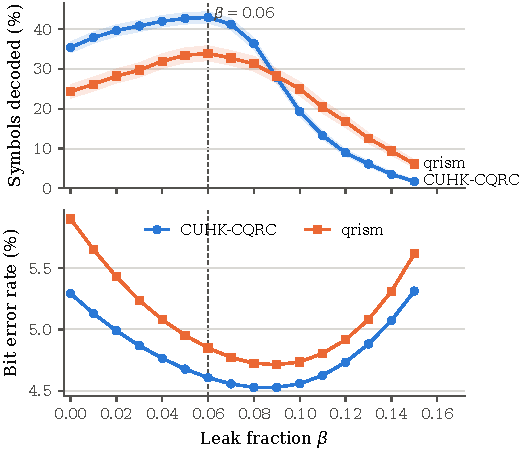
\includegraphics[width=\columnwidth]{generated/fig_beta.pdf}
\caption{Leak fraction $\beta$ against symbol decode rate with its 95\% Wilson band (top)
and pre-correction bit error rate (bottom), RDA shrink $\lambda=0.5$. $\beta=0$ is RDA
without leak inversion. Each dataset's photographs are those localized at the right
version.}
\label{fig:beta}
\end{figure}

Fig.~\ref{fig:beta} sweeps $\beta$ from 0 to 0.15. On each dataset separately the decode
rate peaks at $\beta=0.06$: \HiqCodeChosen\% on CUHK-CQRC against \HiqCodeNoDeblur\%
without leak inversion, and \QrCodeChosen\% on the qrism dataset against
\QrCodeNoDeblur\%. Because both datasets select the same value, choosing $\beta$ on one
and testing on the other costs nothing. The optimum is narrow but not sharp: $\beta=0.05$
cannot be told apart from 0.06 ($p\HiqPFive$ and $p\QrPFive$), while 0.04 ($p\HiqPFour$,
$p\QrPFour$) and 0.07 ($p\HiqPSeven$, $p\QrPSeven$) are worse on both datasets. Past 0.08
the noise gain dominates and decoding collapses, to \HiqCodeTwelve\% and \QrCodeTwelve\%
at $\beta=0.12$.

The bit error rate does not peak where decoding does. At $\beta=0.06$ it falls from
\HiqBerNoDeblur\% to \HiqBerChosen\% on CUHK-CQRC and from \QrBerNoDeblur\% to
\QrBerChosen\% on qrism, but it keeps falling, to $\beta=\HiqBerMinBeta$ on CUHK-CQRC and
\QrBerMinBeta{} on qrism. Our reading is that the photographs that can be decoded at all
want less correction than those that cannot. On
the qrism dataset the bit error rate of 20\,px symbols is lowest at
$\beta=\QrBerMinBetaPxTwenty$, next to their decode optimum, while 12\,px and 8\,px
symbols, which rarely decode, are best served by $\beta=\QrBerMinBetaPxTwelve$ and
\QrBerMinBetaPxEight. Those symbols pull the pooled bit error rate toward larger $\beta$
without adding decoded symbols. The per-photograph optical estimate shows the same split:
it has the lowest bit error rate of any setting on both datasets, yet on CUHK-CQRC it
decodes fewer symbols than the fixed value (\HiqCodeOptical\% against \HiqCodeChosen\%,
$p\HiqPOptical$); on qrism the two tie (\QrCodeOptical\% against \QrCodeChosen\%,
$p\QrPOptical$).

Blue is the weakest channel on both datasets. At $\beta=0.06$ its bit error rate is
\HiqBerChosenB\% on CUHK-CQRC against \HiqBerChosenR\% and \HiqBerChosenG\% for red and
green, and \QrBerChosenB\% on qrism against \QrBerChosenR\% and \QrBerChosenG\%. HiQ
reports the same for its third layer~\cite{yang2018hiq}. Since a qrism symbol decodes only
when all three channels do, the blue channel bounds its decode rate.

\subsection{Covariance shrink}

% Generated by scripts/make_tables.py. Do not edit.
\begin{table}[t]
\centering
\small
\caption{Symbol decode rate (\%) against the RDA shrink $\lambda$, without leak
inversion ($\beta=0$) and with it ($\beta=0.06$).}
\label{tab:shrink}
\begin{tabular}{@{}lrrrr@{}}
\toprule
 & \multicolumn{2}{c}{CUHK-CQRC} & \multicolumn{2}{c}{qrism} \\
\cmidrule(lr){2-3}\cmidrule(l){4-5}
$\lambda$ & $\beta=0$ & $0.06$ & $\beta=0$ & $0.06$ \\
\midrule
0.0 (QDA) & 21.2 & 28.6 & 12.9 & 17.8 \\
0.2 & 33.6 & 39.5 & 21.5 & 31.6 \\
0.4 & 35.5 & 42.5 & 23.5 & 33.3 \\
0.5 (used) & \textbf{35.4} & \textbf{42.9} & \textbf{24.3} & \textbf{33.9} \\
0.6 & 34.9 & 43.1 & 24.6 & 33.9 \\
0.8 & 33.7 & 42.8 & 24.3 & 33.0 \\
1.0 (LDA) & 32.2 & 41.9 & 22.3 & 30.0 \\
\bottomrule
\end{tabular}
\end{table}


Table~\ref{tab:shrink} crosses the RDA shrink $\lambda$ with $\beta$. Decode rates are flat
for $\lambda$ between 0.4 and 0.7 and fall at both ends. With leak inversion, QDA decodes
\HiqCodeQda\% on CUHK-CQRC ($p\HiqPQda$ against $\lambda=0.5$) and \QrCodeQda\% on qrism
($p\QrPQda$): per-class covariances estimated from few samples (17 for black on
CUHK-CQRC), then amplified by the correction, generalize poorly. LDA loses less, \HiqCodeLda\% ($p\HiqPLda$)
and \QrCodeLda\% ($p\QrPLda$). The best cell of the full grid is \HiqGridBest{} on CUHK-CQRC
(\HiqGridBestCode\%, $p\HiqGridBestP$ against $\lambda=0.5$) and \QrGridBest{} on qrism. For
every $\lambda \geq 0.3$ the best $\beta$ is \GridBestBetaRange, so the two parameters can
be set independently.

\subsection{Module size and capture condition}

% Generated by scripts/make_tables.py. Do not edit.
\begin{table}[t]
\centering
\small
\caption{qrism dataset: symbol decode rate (\%) by module size and capture condition,
without leak inversion, at $\beta=0.06$, and at the best fixed $\beta$ for that
group. $n$ is localized photos.}
\label{tab:breakdown}
\begin{tabular}{@{}lrrrrr@{}}
\toprule
Group & $n$ & $\beta=0$ & $0.06$ & best $\beta$ & at best \\
\midrule
0.34 mm & 263 & 52.1 & 46.0 & 0.03 & 54.8 \\
0.5 mm & 1061 & 9.3 & 18.5 & 0.08 & 19.8 \\
0.84 mm & 1136 & 43.8 & 56.0 & 0.06 & 56.0 \\
\midrule
regular & 1024 & 27.8 & 39.8 & 0.05 & 40.5 \\
daylight & 271 & 46.1 & 41.3 & 0.01 & 49.1 \\
flashlight & 458 & 14.0 & 28.4 & 0.10 & 31.0 \\
monitor & 75 & 90.7 & 89.3 & 0.01 & 92.0 \\
close & 28 & 82.1 & 85.7 & 0.02 & 85.7 \\
wb-cool & 23 & 30.4 & 47.8 & 0.10 & 65.2 \\
wb-neutral & 145 & 11.7 & 35.9 & 0.10 & 55.2 \\
wb-warm & 173 & 4.0 & 16.2 & 0.06 & 16.2 \\
\bottomrule
\end{tabular}
\end{table}


Table~\ref{tab:breakdown} breaks the qrism results down. The best $\beta$ grows as modules
shrink: \QrBestBetaPxTwenty{} at 20\,px, \QrBestBetaPxTwelve{} at 12\,px and
\QrBestBetaPxEight{} at 8\,px. This is what a blur of fixed width in pixels predicts, since
it covers a larger fraction of a smaller module. At 8\,px almost nothing decodes, at most
\QrBestCodePxEight\%. Capture conditions move the optimum as well: daylight photographs do
best at $\beta=\QrBestBetaDaylight$ (\QrBestCodeDaylight\% against \QrCodeChosenDaylight\%
at 0.06), while the neutral white-balance condition does best at \QrBestBetaWbNeutral{} and
the flash condition at \QrBestBetaFlashlight. These per-group optima are chosen on the photographs they are
scored on, so they overstate what a per-group $\beta$ would gain; they show that a single
$\beta$ is a compromise across conditions.

\subsection{Comparison with the HiQ decoder}
\label{sec:hiq}

% Generated by scripts/make_tables.py. Do not edit.
\begin{table}[t]
\centering
\small
\caption{End-to-end decoders on HiQ's test split of CUHK-CQRC, paired by photo. Each decoder uses its own
localization and sampling. CMI, corrected: all five CMI weights, with the neighbors HiQ's
sampler gathers (two of four on most modules). Disc.: photos only ours decoded / only HiQ
decoded; every difference has exact McNemar $p<10^{-127}$.}
\label{tab:paired}
\setlength{\tabcolsep}{4pt}
\begin{tabular}{@{}lrcr@{}}
\toprule
Decoder & Symbol \% & 95\% CI & Disc. \\
\midrule
\multicolumn{4}{@{}l}{\emph{Localized by both ($n=3404$)}} \\
Ours, $\beta=0.06$ & 50.1 & [48.4, 51.7] & \\
HiQ QDA & 26.0 & [24.6, 27.5] & 926/108 \\
HiQ QDA + CMI, corrected & 29.5 & [28.0, 31.0] & 824/123 \\
HiQ layered SVM & 25.5 & [24.1, 27.0] & 931/95 \\
\midrule
\multicolumn{4}{@{}l}{\emph{All photos ($n=5381$)}} \\
Ours, $\beta=0.06$ & 35.3 & [34.0, 36.5] & \\
HiQ QDA & 17.2 & [16.2, 18.3] & 1119/149 \\
HiQ QDA + CMI, corrected & 19.5 & [18.4, 20.5] & 1017/167 \\
HiQ layered SVM & 16.7 & [15.7, 17.7] & 1124/126 \\
\bottomrule
\end{tabular}
\end{table}


This comparison uses only HiQ's test split, so no photograph HiQ's models were trained on is
scored. Of its \PairTest{} photographs the HiQ decoder localizes \PairHiqLocalized{} and ours
\PairOursLocalized; \PairBoth{} are localized by both, \PairCommon{} of them at the same
version. Table~\ref{tab:paired} compares the decoders on these photographs and
on all photographs, counting a photograph that a decoder does not localize as a failure.
On the common set our decoder reads \PairCommonOurs\% of symbols against \PairCommonHiq\%
for HiQ's best configuration, QDA with the corrected CMI. It leads in all
\PairVersionsTotal{} symbol versions and all \PairFoldersTotal{} capture folders. Without
leak inversion it reads \PairCommonOursNoDeblur\%, still ahead of HiQ.

The HiQ classifiers were also timed on the same machine, over the same span as ours
(Section~\ref{sec:method}): \HiqTimeLsvmNs\,ns per module for the layered SVM,
\HiqTimeQdaNs\,ns for QDA and \HiqTimeQdaCmiNs\,ns for QDA with the corrected CMI, against
\TimeChosenNs\,ns for ours. These figures do not isolate the algorithms. HiQ runs as
JIT-compiled Java and ours as Rust, which favors ours; HiQ fits nothing per photograph while
our time includes the fit, which favors HiQ. They do show that the costs are of the same order:
ours falls between HiQ's layered SVM and its QDA without any training, and the layered SVM,
the only faster one, decodes \PairCommonLsvm\% of the common set.

One qualification applies. Each decoder uses its own localization and module sampling, so
the gap combines color recovery and sampling; a comparison of the classifiers alone needs
HiQ's classifier run on our samples. \todo{run HiQ's QDA and corrected CMI on the library's
samples, or state the claim as end-to-end only}

\section{Limitations}
\label{sec:limitations}

A single $\beta$ is a compromise. The best value depends on module size in pixels and on
lighting (Table~\ref{tab:breakdown}), and the per-photograph estimates we tried do not
reliably beat the fixed value. Estimating $\beta$ from a photograph in a way that tracks
decodability rather than bit error rate is open.

Calibration assumes the function patterns are intact. Glare, damage or occlusion on a
finder or alignment pattern corrupts the samples the whole photograph is fitted on.

Symbols with 8\,px modules almost never decode, and none of the oblique-view photographs
is localized, so neither condition informs the comparison of color recovery methods.

Each module is read from one pixel at its projected center. Averaging several pixels may
reduce noise but would also mix in more of the neighbors that leak inversion removes; we
have not measured this trade-off.

The comparison with HiQ is end to end (Section~\ref{sec:hiq}) and does not separate color
recovery from localization and sampling.

\section{Conclusion}
\label{sec:conclusion}

Color recovery for multiplexed QR codes does not need offline training. Each photograph is
fitted on its own function patterns: a closed-form inverse of the leak between edge-adjacent
modules, with one fixed fraction $\beta=0.06$, followed by regularized discriminant analysis
with shrink $\lambda=0.5$. These values were chosen on each dataset separately; they are the
best setting on the qrism dataset and statistically tied with the best on CUHK-CQRC
($p\HiqGridBestP$). At these values the method decodes \HiqCodeChosen\% of localized symbols
on CUHK-CQRC and \QrCodeChosen\% on the qrism dataset, and every baseline decodes fewer on
both. Given the same module samples on HiQ's test split, it decodes \PortOursCode\% of symbols
against \PortCmiCode\% for the best of HiQ's trained classifiers, at \TimeChosenNs\,ns per
module including the fit.

Color codes have been proposed for file transfer between phones without a
network~\cite{toh2016colorqr}, for validation data on small product labels such as medicine
packs that must be checked off-line~\cite{melgar2019hd2dc}, for encrypted payloads carried
with their signatures~\cite{wahsheh2026rgb}, and for hidden traceability and
anti-counterfeiting layers beside a layer that standard readers
decode~\cite{huang2022mc2d,huang2023halftone}. In these uses the printer, display and phone
are often not known in advance. Our method assumes nothing about them, only that the
function patterns are intact: it is fitted to each photograph without training data,
recovers the colors of a version-40 symbol in \TimeChosenVforty\,ms, and was evaluated on
both printed and displayed symbols. The decode rates above are for single photographs; a
phone scanner sees many frames per second and could retry on later ones, but we have not
measured how often this helps.

The fixed $\beta$ is the main compromise: its best value shifts with module size, capture
distance and lighting, and choosing it per photograph in a way that tracks decodability rather than
bit error rate remains open.
The Rust implementation is available at \url{https://github.com/mohnishsalian0/qrism}, and
the qrism dataset is released with its source renders.


\bibliographystyle{IEEEtran}
\bibliography{refs}

\end{document}
